% Diese Zeile bitte -nicht- aendern.\pgfplotsset{compat=1.15}
\documentclass[course=erap]{aspdoc}
\graphicspath{ {./} }

%%%%%%%%%%%%%%%%%%%%%%%%%%%%%%%%%
%% TODO: Ersetzen Sie in den folgenden Zeilen die entsprechenden -Texte-
%% mit den richtigen Werten.
\newcommand{\theGroup}{140} % Beispiel: 42
\newcommand{\theNumber}{A208} % Beispiel: A123
\author{Tianhao Gu \and Zhongfang Wang \and Julien Escaig}
\date{Wintersemester 2023/24} % Beispiel: Wintersemester 2019/20
%%%%%%%%%%%%%%%%%%%%%%%%%%%%%%%%%

% Diese Zeile bitte -nicht- aendern.
\title{Gruppe \theGroup{} -- Abgabe zu Aufgabe \theNumber}

\begin{document}
\maketitle

\section{Einleitung}

\par
Das Ziel dieser Projektarbeit ist es, einen Algorithmus in C zu entwickeln, der ein farbiges Bild in ein Graustufenbild umwandelt und anschließend die Helligkeit des Graustufenbilds mithilfe der Gammakorrektur anpasst.

\par
Als Eingabe akzeptiert Unser Programm nur PPM-Dateien des Typs P6. P6 bezieht sich dabei auf das Binärformat der Pixeldaten.  Diese besteht aus einem Header mit Metadaten, worauf die Pixel-Informationen folgen. Im Datenteil der PPM Datei gibt es für jeden Pixel genau drei Werte, die jeweils die Stärke der Farben Rot, Grün und Blau speichern. Je größer der Wert desto stärker ist die Farbe in einem bestimmten Pixel vertreten. Unterhalb ist ein einfaches Beispiel eines solchen Bildes.

\begin{figure}[h]
\begin{minipage}{0.45\textwidth}
\centering
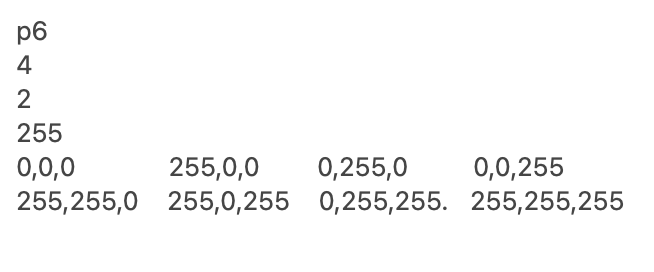
\includegraphics[width=\textwidth]{Bilder/demograph.png}
\caption{ein Beispiel für P6 PPM}
\end{minipage}
\hfill
\begin{minipage}{0.45\textwidth}
\centering

\includegraphics[width=\textwidth]{Bilder/demograph.ppm.png}
\caption{erzeugt durch den Beispielcode}
\end{minipage}
\end{figure}

\par
Die erste Phase des Projekts ist die Graustufenkodierung.Dafür verwenden wir die Formel (1) unten. Dabei wird der gewichtete Durchschnitt der Rot-, Grün- und Blau-Werte jedes Pixels ermittelt. Ein Beispiel ist in Abbildung 3 zu sehen. 
\begin{equation}
D(x,y)=\frac{a*R+b*G+c*B}{a+b+c}
\end{equation}


\begin{figure}[h]
\centering

\includegraphics[width=0.2\textwidth]{Bilder/gamma1.pgm.png}
\caption{Graustufen Konvertierung von Abbildung2}
\end{figure}

\par
Im zweiten Teil der Aufgabe befassen wir uns nun mit einem anderen Aspekt des menschlichen visuellen Systems (HVS) und zwar der Helligkeit. Diese hat einen großen Einfluss darauf, wie natürlich ein Bild auf uns Menschen wirkt. Die Gammakorrektur ändert die Helligkeit bzw. den Kontrast eines Bildes, und hängt von der Wahl des $ \gamma $ Parameters ab.Bei diesem Algorithmus wird die Gammakorrektur durch folgende mathematische Formel (2) bestimmt. Die Werte D'(x,y) ergeben die Intensität der Graustufenkodierung für alle Pixel (x,y). Ein kleinerer Gammawert führt zu einem helleren Bild, während ein größerer Gammawert zu einem dunkleren Bild führt.

\begin{equation}
D'(x,y)={\left( \frac{D(x,y)}{255} \right)}^{\gamma}*255
\end{equation}

\par
Um den Effekt der Gammakorrektur zu visualisieren, betrachten wir nochmal die Abb.3. Unterhalb kann man 3 verschiedene „Helligkeits-Versionen“ von Abb.3 vergleichen.

\begin{figure}[h]
\begin{minipage}{0.3\textwidth}
\centering

\includegraphics[width=\textwidth]{Bilder/gamma0.1.pgm.png}
\caption{Gamma=0.1}
\end{minipage}
\hfill
\begin{minipage}{0.3\textwidth}
\centering

\includegraphics[width=\textwidth]{Bilder/gamma1.pgm.png}
\caption{Gamma=1}
\end{minipage}
\hfill
\begin{minipage}{0.3\textwidth}
\centering

\includegraphics[width=\textwidth]{Bilder/gamma10.pgm.png}
\caption{Gamma=10}
\end{minipage}
\end{figure}

\par
Die Hauptfunktion unsere Programms erhält 6 Parameter. Zwei davon sind \texttt{input\_file\_name} und \texttt{output\_file\_name}, welche die Pfade des Eingabebildes und des Ausgabebildes repräsentieren. Der Parameter \texttt{version} vom Datentyp \texttt{int} gibt die Version an. Der Parameter \texttt{benchmark\_number} repräsentiert die Anzahl der Benchmark-Zyklen. Die Parameter \texttt{a}, \texttt{b}, und \texttt{c} vom Datentyp \texttt{float} stellen die RGB-Gewichte für die Graustufenumwandlung dar. Schließlich erhält die Funktion noch einen Parameter \texttt{\_gamma} vom Datentyp \texttt{float}, der für den Gammawert steht.

\par
Obwohl die oben genannten Parameter zusätzlich zu den Ein- und Ausgängen standardmäßig mit sinnvollen Defaultwerten besetzt sind, kann der Nutzer diese Parameter auch selbst mit spezifischen und sinnvollen Werten ersetzen. Wenn die gesetzten Werte nicht sinnvoll sind, wird eine Fehlermeldung ausgegeben und das Programm wird beendet.Hier ist eine Übersicht an Optionen, die der Nutzer beim Aufrufen des Programms setzrn kann:

\begin{itemize}
\item Option \emph{-V<Zahl>} Die Option -V 0 ist die Standardimplementierung. -V 1 steht für die Implementierung V1 mit Taylorreihe. -V 2 steht für die Implementierung V2 mit SIMD. Andere Werte sind nicht erlaubt.
\item Option \emph{-B<Zahl>} Falls gesetzt, wird die Laufzeit der angegebenen Implementierung gemessen und ausgegeben. Das Argument gibt die Anzahl an Wiederholungen des Funktionsaufrufs an. Es darf nicht kleiner als 1000 sein.
\item Positionalem Argument \emph{<Dateiname>} Der Pfad zur Eingabedatei ist ein obligatorischer Parameter. Falls dieser ungültig ist, wird eine Fehlermeldung ausgegeben und das Programm wird beendet.
\item Option \emph{-o<Dateiname>} Der Pfad zur Ausgabedatei ist ein obligatorischer Parameter. Falls dieser ungültig ist, wird eine Fehlermeldung ausgegeben und das Programm wird beendet.
\item Option \emph{-{}-coeffs<FP Zahl>,<FP Zahl>,<FP Zahl>} Die drei Argumente müssen stets nicht-negativ sein und dürfen nicht den Wert Infinity und NaN annehmen. Ihre Summe darf auch nicht 0 betragen.
\item Option \emph{-{}-gamma<Floating Point Zahl>} Der Gammawert kann nicht negativ sein. Wenn diese Option nicht gesetzt wird, wird standardmäßig der Wert 1 verwendet.
\item Option \emph{-h|-{}-help} Eine Beschreibung aller Optionen des Programms und Verwendungsbeispiele werden ausgegeben und das Programm danach beendet. 
\end{itemize}

\section{Lösungsansatz}

\par
Wir betrachten nun die Implementierung des Programms. Beim Aufrufen des Programms muss der Benutzer die Eingabedatei und die Ausgabedatei angeben, sonst erhält er eine Fehlermeldung über unvollständige Parameter. Zusätzlich hat der Benutzer die Möglichkeit, beim Ausführen des Programms andere Optionen auszuwählen,Zunächst ruft die main-Funktion parse\_options(argc, argv) auf, welche die Methode GETOPT\_LONG(3) verwendet, um die Parameter von der Eingabe von dem Nutzer zu erhalten. Anschließend werden switch-case-Anweisungen zur Verarbeitung und Speicherung der jeweiligen Parameter verwendet. getopt\_long ist eine Funktion in C, die zum Parsen von Befehlszeilenparametern verwendet wird. Sie kann kurze Optionen (z.B.-o) und lange Optionen (z.B.--coeffs) verarbeiten. 

\par
Gemäß der Netpbm-Dateibeschreibung ist die ppm-Datei in zwei Teile unterteilt: Metadaten und Pixelbereich. Für die Formatierung dieser beiden Teile gibt es entsprechende Regeln. Zu beachten ist auch, dass in den Metadaten ein Kommentar an beliebiger Stelle eingefügt werden kann. Daher wird beim Lesen der Metadaten in der ppm-Datei ein Zustandsautomat entworfen und verwendet, um mit möglichen Randfällen fertig zu werden.Der Zustandsautomat für das Lesen der Metadaten in der ppm-Datei ist in den folgenden beiden Diagrammen dargestellt.Abbildung 1: Lesen von P6 in den Metadaten und Verarbeitung möglicher Kommentare. state N zeigt an, dass ein Kommentar eingegeben wurde. state N kann nur durch das Lesen eines LF oder CR verlassen werden.Abbildung 2: Dieser Zustandsautomat wird zum Lesen von width, height und maxval und zur Verarbeitung möglicher Kommentare verwendet. state N zeigt an, dass ein Kommentar eingegeben wurde. state N kann nur durch das Lesen eines LF oder CR verlassen werden.

\begin{figure}[h]
\centering
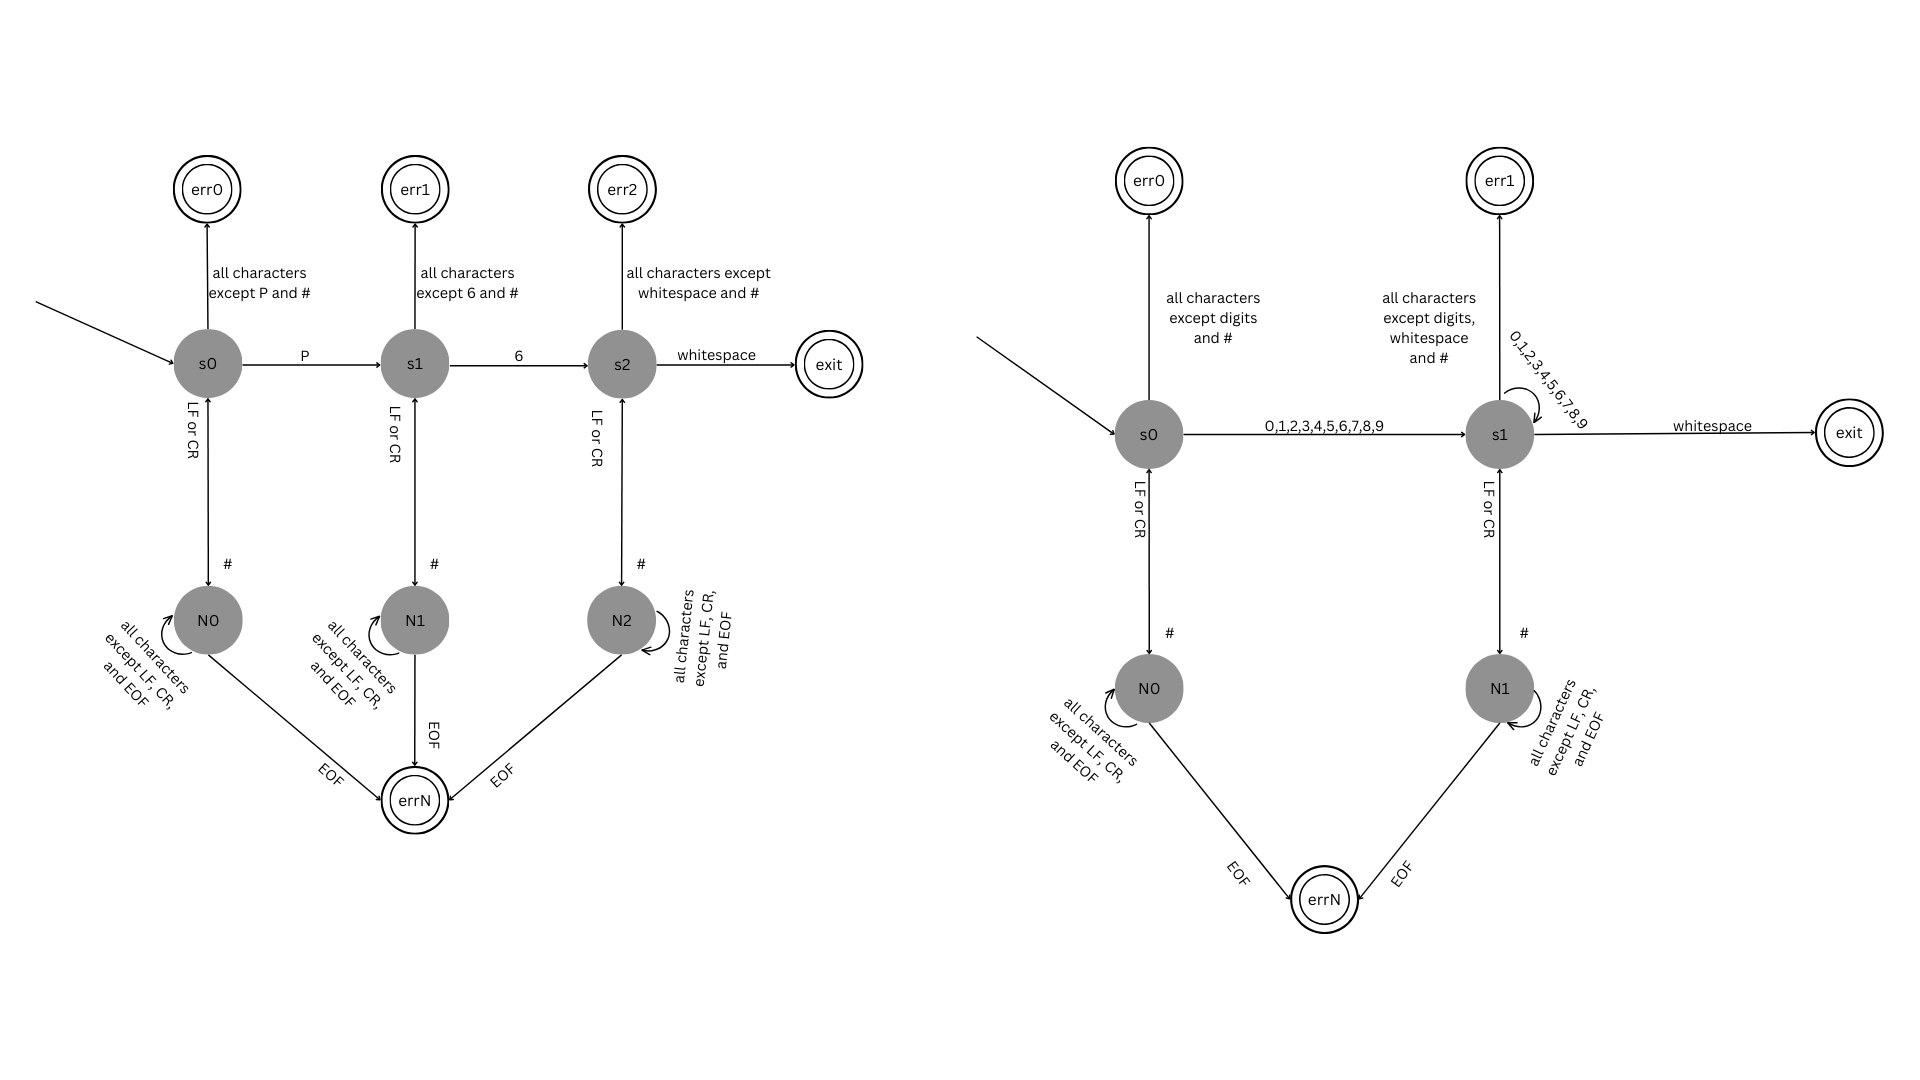
\includegraphics[width=1\textwidth]{Bilder/auto.png}
\caption{Zustandsautomat für das Lesen der Metadaten in der ppm-Datei}
\end{figure}

\par
Bei der Versionsnummer kann der Benutzer zwischen 0, 1 oder 2 wählen. Bei Version 0 und 1 handelt es sich um Algorithmen mit  sequentiellen Anweisungen, Version 2 mit SIMD Instruktionen. Wenn der Nutzer keine Version angibt, wird Version 0 als default durchgeführt.

\par
Bei der Implementation von V0 und V1 werden die drei Farben jedes Pixels beim Lesen der Eingabedatei in der originalen Reihenfolge gespeichert. Wenn V2 verwendet wird, werden beim Einlesen die drei Farben jedes Pixels getrennt gespeichert. Dadurch werden drei Speicherbereiche im Heap erstellt, die jeweils für eine bestimmte Farbe alle Pixelwerte in fortlaufender Reihenfolge speichern. In main wird eine Switch-Anweisung verwendet, um verschiedene Funktionen abhängig von der gewählten Versionen aufzurufen. 

\par
In allen aufgerufenen Funktionen wird zunächst die Eingabedatei gelesen und dann basierend auf den Metadaten der Eingabedatei Speicher für die Eingabe und Ausgabe allokiert. Die Allokation des Speichers wird durch den Aufruf einer neuen Funktion implementiert. In V2, der SIMD-Implementierung, wird aligned\_alloc() verwendet, um Speicher zu reservieren (cite). Die Startadresse des Speichers wird auf ein Vielfaches von 16 ausgerichtet und erhöht damit die Geschwindigkeit des Ladens von Speicher in die xmm-Register. Anschließend werden verschiedene Versionen von gamma\_correct()aufgerufen.

\par
In V0 und V1 wird zunächst die Graustufenkonvertierung für jeden Pixel sequentiell berechnet. V2 verwendet SIMD-Anweisungen, welche es ermöglichen die Graustufenwerte von vier Pixeln gleichzeitig zu berechnen. Nachdem die Graustufenwerte der Pixel berechnet wurden, verwenden V0 und V2 die pow-Funktion der math.h-Bibliothek,um die Graustufenwerte nach der Gammakorrektur für jedes Pixel sequenziell zu berechnen. V1 verwendet keine Bibliotheksfunktionen, sondern implementiert die Taylor-Entwicklung.

\par
Die Taylor Entwicklung ist eine lokale Approximation eines Funktionswertes der Form $f(x) = f(a) + f'(a)(x-a) + \frac{{f''(a)(x-a)^2}}{2!} + \frac{{f'''(a)(x-a)^3}}{3!} + \ldots + \frac{{f^n(a)(x-a)^n}}{n!} + R_n(x) $ Wir verwenden den Fall $a=1$ und erhalten die Formel:

\begin{equation}
f(x) = 1 + \frac{(x-1)^1}{1!} (\gamma) + \frac{(x-1)^2}{2!} (\gamma)(\gamma-1)  + \cdots + \frac{(x-1)^n}{n!} \prod_{i=0}^{n-1} (\gamma-i) + R_n(x)
\end{equation}

\par
Bei Gamma-Werten größer als der magischen Zahl 67075968 ist das Ergebnis für einen anderen Basiswert als 1 immer 0 (Unterlauf). Daher wird darauf geachtet, dass die nachfolgenden Gammawerte kleiner als diese magische Zahl sind. Im Falle eines Basiswerts von 1 wird dies als Sonderfall behandelt, und das Ergebnis bleibt unabhängig vom Gamma-Wert immer 1.

\par
Eine Beobachtung für Formel (1) ist, dass unser Base D(x,y) ist immer eine Zahl zwischen 0 und 1 ist. Gamma ist auf die Bedingung beschränkt, dass es größer als 0 und nicht Infinity oder NaN ist. Bei der Entwicklung haben wir festgestellt, dass die Fakultäten von Gamma bei größeren Gammawerten leicht zu einem Overflow führt, denn wie müssen die Fakultät von Gamma berechnen.Nachdem wir den Fall behandelt haben, dass Gamma zu groß ist, haben wir Gamma in eine ganze Zahl und eine Dezimalzahl zerlegt und separat berechnet,um immer noch mögliche Overflows zu vermeiden.

\par
Für Den Ganzzahlanteil ist unser Design Gedanke, den Exponenten in eine binäre Zahl umzuwandeln und dann zu zerlegen. Im folgenden Beispiel wird die 29. Potenz von 0,79 berechnet

\[
29 = 1 \cdot 2^0 + 0 \cdot 2^1 + 1 \cdot 2^2 + 1 \cdot 2^3 + 1 \cdot 2^4
\]
\[
0.79^{29} = 0.79^{2^0} \cdot 0.79^{2^2} \cdot 0.79^{2^3} \cdot 0.79^{2^4}
\]

\par
Da Gamma eine Fließkommazahl ist, ist der Ganzzahlanteil maximal 67075968, also zwischen $2^{25}$ und $2^{26}$, so dass wir unabhängig vom Exponenten höchstens 26 Schleifen benötigen.

\par
!!!!Die Graustufenwerte nach der Gammakorrektur werden über einen weiteren Funktionsaufruf in die Ausgabedatei geschrieben. Bevor alle Ressourcen freigegeben werden, wird gamma\_correct() wiederholt ausgeführt, wenn der Benutzer die Option \-B in den Optionen aktiviert hat. Die Zeit wird zu Beginn und am Ende des Zyklus aufgezeichnet. Diese Laufzeit des Zyklus wird später für die Leistungsanalyse verwendet.

\par
!!!!Am Ende der main\-Funktion müssen alle Ressourcen freigegeben werden. Um Speicherlecks zu vermeiden, verwenden wir die free\-Funktion und fclose, um den Speicherbereich freizugeben. Zusätzlich wird an sämtlichen Stellen in main\-Funktion, an denen eine Allocation oder eine IO\-Operation durchgeführt wird, überprüft, ob sie erfolgreich war. Wenn der entsprechende Vorgang fehlschlägt, werden alle Ressourcen des aktuellen Programms freigegeben und eine Fehlermeldung in stderr ausgegeben. Danach wird das Programm mit dem Status EXIT\_FAILURE beendet.

\par
Das Programm verteilt alle Funktionen sinnvoll auf die verschiedenen Funktionen. Jede Funktion ist angemessen groß, logisch korrekt, leicht zu warten und vermeidet Blob Muster.

\section{Genauigkeit}
\par
In diesem Teil wird die Genauigkeit bzw. Korrektheit des Algorithmus untersucht. Dafür ist erst einmal zu klären, welches der beiden Konzepte bei dieser Problemstellung sinnvoll anwendbar ist.

\par
Da der Algorithmus zwischendurch mit Float-Werten arbeitet, kann es zu Ungenauigkeiten kommen, da nicht alle Zahlen als Float darstellbar sind. Der maximale Fehler bei 32 bit Float beträgt ungefähr xxx. Diese mögliche Ungenauigkeit wird bei der Gammakorrektur noch verstärkt (Die Ungenauigkeit hängt zudem noch von der internen Implementation der arithmetischen Operationen ab). Obwohl der Fehler immer noch sehr klein ist, kann es bei der Rundung zu Integern zu unterschiedlichen Werten kommen. Für das menschliche Auge macht es keinen Unterschied. Die Bilder sehen identisch aus, obwohl nicht alle Integerwerte in der PGM Datei übereinstimmen. Aus diesen Gründen macht es Sinn, das resultierende Bild auf Genauigkeit anstatt auf Korrektheit zu überprüfen.

\par
Im Folgenden werden die 2 Teile des Programms erstmal getrennt voneinander auf Genauigkeit geprüft. Beginnen wir also mit der Graustufenkodierung.

\par
Um unsere Implementierung der Graustufenkodierung auf Genauigkeit zu überprüfen, verwenden wir die von Netpbm bereitgestellte Funktion “ppmtopgm” als Referenz. Dazu haben wir eine Funktion entworfen die zwei PGM Dateien als Input nimmt und die betragsmäßige Abweichung über alle Pixel berechnet. Die Grafik1 zeigt unsere Ergebnisse für verschiedene PGM Dateien unterschiedlicher Größe.

\par
Diese Abweichungen können jedoch niemals mit bloßem Auge erkannt werden, wie Abbildung 4 demonstriert.

\par
Nun folgt die Genauigkeitsanalyse des zweiten Teils des Programms. Diese wird erneut in mehrere Teile aufgeteilt. Dafür überprüfen wir die Genauigkeit der Pow()-Funktion, die der Taylorreihe und abschließend noch die der SIMD Implementation. Als Referenz der für das Resultat nach der Gammakorrektur verwenden wir die Funktion “gammakorrekt” des Netpbm Packages. In der Grafik2 kann man nun die Abweichung unserer Implementierung von der Netpbm-Implentierung beobachten.

\par
Nun beschäftigen wir uns mit der Genauigkeit der Taylorreihe. Die Taylorreihe ist eine Approximation, die erst bei unendlich vielen Gliedern exakt wird. In unserer Implementation der Taylorreihe brechen wir die Berechnung der Taylorreihe ab, sobald das nächste Reihenglied betragsmäßig kleiner als 0.00000001 ist. Dies lässt vermuten, dass die Abweichung bei dieser Implementation größer sein wird, als beim Verwenden der Pow-Funktion. In Grafik3 ist klar zu erkennen, dass es durch die Approximation der Taylorreihe insgesamt zu einer höheren Abweichung kommt.


\par
Abschließend betrachten wir noch die SIMD Implementation. Es ist zu erwarten, dass es zu keinem Unterschied in der Abweichung kommt, da die gleichen Operationen auf den gleichen Variablen durchgeführt werden. Grafik4 unterstreicht diese Hypothese.

\par
Das Resultat wird in einer Datei des PGM-Formats gespeichert. Logischerweise wählen wir PGM als Format für unsere Outputdatei, da es Graustufenbilder speichert. Jeder Pixelwert liegt zwischen 0 und dem maximalen Grauwert. wobei 0 normalerweise Schwarz darstellt, der maximale Grauwert Weiß. Alle Werte dazwischen ergeben die verschiedenen Grautöne. Der maximale Grauwert ist üblicherweise 255 (8 Bits). Bei der Konvertierung ist noch zu beachten, wie die "Gewichte" von RGB gewählt werden.

\section{Performanzanalyse}


\section{Zusammenfassung und Ausblick}
\par
Bei\cite{vmintromiami} diesem Projekt ging es darum, eine Graustufen-Kodierung und Gammakorrektur selber zu programmieren. Das Umsetzen der Graustufen-Kodierung war relativ einfach, genau wie die Implementierung mit der Pow-Funktion. Die Aufgabe erhielt eine neue Stufe an Komplexität, sobald es zur Implementierung mit der Taylorreihe und der SIMD Implementierung kommt. Die Taylorreihe führt zu einer geringeren Genauigkeit. Die SIMD-Funktion hat zu einer höhere Performanz von etwa … Prozent geführt. Abschließend kann man sagen, dass dieses Projekt einen interessanten Einblick in verschiedene Bildformate, das Approximieren mit Hilfe der Taylorreihe und das Optimieren mit Hilfe von SIMD-Intrinsics geliefert hat.

% TODO: Fuegen Sie Ihre Quellen der Datei Ausarbeitung.bib hinzu
% Referenzieren Sie diese dann mit \cite{}.
% Beispiel: CR2 ist ein Register der x86-Architektur~\cite{intel2017man}.
\bibliographystyle{plain}
\bibliography{Ausarbeitung}

\end{document}



